\chapter{Analýza výkonnosti a obmedzení }

SVG. vs Canvas 
Počet objektov SVG 

Zložitosť SVG - výpočtový výkon

\url{https://msdn.microsoft.com/library/gg193983(v=vs.85).aspx}

 \begin{figure}[H]
\centering
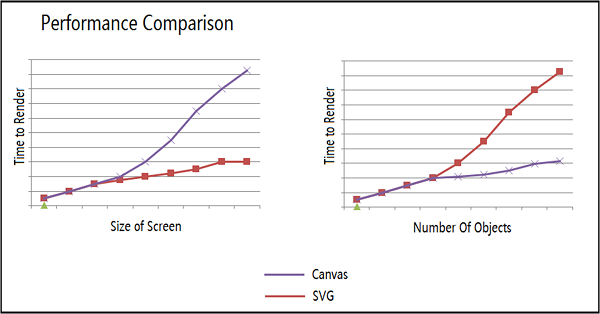
\includegraphics[width=0.7\linewidth]{obrazky/porovnanie}
\caption{Porovnanie výkonnosti Canvas vs. SVG}
\label{fig:podpora}
\end{figure}

Generally, as the size of the screen increases, canvas begins to degrade as more pixels need to be drawn. As the number of objects increases on the screen, SVG begins to degrade as we are continually adding them to the DOM. These measurements are not necessarily accurate and can certainly change depending upon implementation and platform, whether fully hardware accelerated graphics are being used, and the speed of the JavaScript engine.


















%Pre meranie výkonnosti vizualizácie grafických komponentov v reálnom čase zadefinujem v nasledujúce kritéria \begin{itemize}	\item počet komponentov, 	\item čas načítania stránky, 	\item čas vykonania zmeny atribútov v komponentoch.\end{itemize}Testy boli vykonané vo webovom prehliadači Chrome verzia 45 a Firefox verzia 40.  V teste boli použité nasledujúce navrhnuté komponenty:\begin{itemize}	\item teplomer, 	\item prečerpávacia stanica, 	\item trojcestný ventil, 	\item mapa Slovenska, 	\item prepravný pás. \end{itemize}Objekty boli v rovnakom zastúpení v jednom HTML súbore  v počtoch: 1,5,10,25, 50, 100.Ukážka testovacej situácie je na obrázku TODO SCREEN. A výsledky sú uvedené v tabuľke TODO TABULKA. \newpage Alebo vytvorim test -\url{http://jsperf.com/}- kde porovnam SVG smil animaciu s snap.svg.jsktore je v kapitole 4 - strana vtedy bola 20

%
%\url{http://www.sitepoint.com/advanced-snap-svg/}
%Performance Improvements
%
%One way to improve performance when manipulating the DOM is using DocumentFragments. Fragments are minimal containers for DOM nodes. Introduced a few years ago, they allow you to inexpensively manipulate entire subtrees, and then clone and add a whole subtree with n nodes to our page with 2 method calls instead of n. The actual difference is explained in details on John Resig’s blog.
%
%Snap allows for native use of fragments as well, with two methods:
%
%Snap.parse(svg) takes a single argument, a string with SVG code, parses it and returns a fragment that can be later appended to any drawing surface.
%
%Snap.fragment(varargs) takes a variable number of elements or strings, and creates a single fragment containing all the elements provided.
%
%Especially for large svg drawings, fragments can lead to a huge performance saving, when used appropriately.
%
%
%\newpage
%
%%http://www.html5rocks.com/en/tutorials/speed/high-performance-animations/
%
%\url{http://caniuse.com/#feat=svg-html}
%
%
%***********************
%
%Animácia pozície 
%- transform: translate(npx, npy);
%
%Animácia škály 
%- transform: scale(n);
%
%Animácia otáčania
%- transform: rotate(ndeg)
%
%Animácia neprehľadnosti 
%- opacity: 0..1;
%
%*************************
%
%%\url{http://www.svgopen.org/2008/papers/74-HighPerformance_GML_to_SVG_Transformation_for_the_Visual_Presentation_of_Geographic_Data_in_WebBased_Mapping_Systems/}
%
%
%\textbf{Transformation}
%\textit{scale}(sx, sy) - zmenim veľkosť tvaru na danane suradnice, 
%\textit{translate}(tx, ty) - presuniem na ine miesto - zmenim suradnice 
%
%%\url{https://developers.google.com/web/fundamentals/performance/rendering/optimize-javascript-execution?hl=en}
%
%Podpora svg v prehliadačoch
%\url{http://caniuse.com/#feat=svg}
%
%\url{http://www.schepers.cc/svg/blendups/embedding.html}